\documentclass[twocolumn,showpacs,preprintnumbers,amsmath,amssymb,floatfix]{revtex4-1}
\usepackage{mysty}
\usepackage{amsmath}
\usepackage{subcaption}
%\usepackage[caption=false]{subfig}


\begin{document}

\title{Data-driven modeling of the low-Atwood single-mode Rayleigh-Taylor instability}

\author{Maxwell Hutchinson}
\affiliation{The Physics Department, University of Chicago, Chicago IL 60637}
\email{maxhutch@uchicago.edu}

\date{\today}

\begin{abstract}
The Rayleigh-Taylor instability (RTI) pervades classical fluid dynamics and is essential to a diversity of phenomena, e.g. salt fingers, thermonuclear flames, and inertial confinement fusion, but remains poorly understood in dissipative systems.
Recently, the single-mode RTI has shown experimentally and numerically to deviate from established potential flow models when the Atwood number was less than $1/2$.
Attempts to explain the deviation, termed re-acceleration, have been ad-hoc and hindered by a dearth of data at late times and high aspect ratios.
This paper present buoyancy-drag and mixing models that include dissipative terms and match the linear theory.
To inform the model, a numerical experiment is performed, simulating a range of Grashof and Schmidt numbers and reaching bubble heights of $17\lambda$.
The model coefficients are estimated by physical argument and then fit to the numerical results.
The model error is less than 2\% for the bubble height and 4\% for the volume of mixed fluid.
An attempt is made to interpret variations in the fit parameters with the Rayleigh and Schmidt numbers, where present, but it is hindered by many of the simulations interacting with the boundaries.
Simulations in higher aspect ratio domains would improve the model.
\end{abstract}

\pacs{}
\maketitle

\section{Introduction}

The Rayleigh-Taylor instability has been the subject of considerable study since its characterization by Lord Rayleigh in the 19th century.
Despite this, many aspects of the non-linear growth remain poorly understood.
Analytic models based on potential flow have been reasonably effective for flows with a large density jump, i.e. Atwood number, $\Delta \rho / \sum \rho$, near unity.
However, recent experiments at low Atwood number have demonstrated a significant departure from the potential flow limit.
The Rayleigh-Taylor front can be seen accelerating past the terminal velocity predicted by potential flow models.
The acceleration persists beyond times which are experimentally accesible, so numerous efforts have been made to compute the late time flow numerically.
Ultimately, the goal is to use these computational experiments to inform a simple model that captures the key features of the flow, as potential flow models do for high Atwood number flows.

This study concerns the dynamics of the single-mode Rayleigh-Taylor instability (smRTI), where the interface between a heavy fluid and a light fluid is perturbed with a single wavelength $\lambda$ and corresponding wavenumber $k$.
If the Atwood number is low, then at early times the interface grows exponentially with a rate given by a linear approximation:
\begin{equation} \elabel{duff0}
\gamma = \sqrt{\frac{A g k}{1 + \pi^{-1/2} k \delta} + \nu^2 k^4} - (\nu + D) k^2,
\end{equation}
where $A$ is the Atwood number,
$g$ is the local acceleration,
$\delta$ is the interface thickness,
$\nu$ is the kinematic viscosity, and
$D$ is the diffusivity.

As the amplitude approaches the wavelength, the linear growth saturates.
At unit Atwood number, the non-linear regime is described by potential flow, which approaches a terminal velocity given by Layzer~\cite{Layzer1955}:
\begin{equation}
v_L = \sqrt{g \lambda}
\end{equation}
(check)
Potential flow models have been extended $A < 1$, with the most successful model by Goncharov~\cite{Goncharov2002}:
\begin{equation}
v_G = \sqrt{A g \lambda}
\end{equation}

Experiments by Wilkinson and Jacobs show that after reaching the velocity given by \eref{goncharov}, low Atwood bubbles unexpectedly accelerate a second time.
This is termed `reacceleration`, with the terminal velocity replaced by a `stagnation velocity`.
Reacceleration was not present in popular potential flow and buoyancy-drag models, and attempts to caputre reacceleration have been the emphasis of recent model development in the low Atwood number regime.

Experiments have thus far been unable to observe more than the onset of the reacceleration phase.
Therefore, the community has turned to numerical studies to compute late-time dynamics.
At least two such efforts have been under-taken, one by Ramaprabu et al and one by Wei and Livescu, leading to slightly different conclusions.
In the study by Ramaprabhu, the flow accelerates to around twice the stagnation velocity and then decelerates back to the stagnation velocity, indicating that reacceleration may be a transient.
In the study by Wei and Livescu, the flow reaccelerates and then breaks up into many small pockets of buoyant fluid, which themselves continue to accelerate at nearly a fixed rate.

Buoyoncy-drag models have been proposed for the multi-mode and single-mode dynamics of the bubble front.
They balance the buoyant force of the bubble with a drag force to predict the front velocity as a function of the characteristic length.
Ramaprabhu proposes an additional forcing term based on the development of a vortex ring at the bubble tip, but relies on observation of the mean vorticity experimentally or in numerical simulations.
There is a need for a predictive model for reacceleration that relies only on the initial conditions.

\paragraph{Outline}
In \sref{model}, we propose a simple buoyancy-drag model for the dynamics of the smRTI.
In \sref{results}, we present a battery of numerical trials.
In \sref{fit}, we evaluate the simple model against numerical results.
In \sref{discuss}, we discuss the strengths and weaknesses of the model, extensions, and potential tests.
Finally, in \sref{conc}, we assess the current state of smRTI and highlight outstanding questions.



\section{Simple model} \slabel{model}

We base our model on the buoyancy-drag models of \cite{Oron2001}:
\begin{equation}
(\rho_1 + \rho_2) \mathcal{V} \ddot{h} = (\rho_2 - \rho_1) g \mathcal{V} - C \dot{h}^2 \rho \mathcal{A}
\end{equation}
where $\rho_1$ and $\rho_2$ are the densities of the light and heavy fluid,
$\mathcal{V}$ is the characteristic volume of the bubble
$g$ is the acceleration,
$C$ is a drag-like coefficient, and
$\mathcal{A}$ is the characteristic cross sectional area of the bubble.
Making the Boussinesq approximation, $\rho_1 \approx \rho_2$ yields:
\begin{equation}
\ddot{h} = A g - \frac{C}{2} \dot{h}^2 \frac{\mathcal{A}}{\mathcal{V}}
\end{equation}
In the self-similar regime there is only one length-scale, so $\mathcal{A}/\mathcal{V} \sim 1 / \lambda$.
However, in the single-mode regime that is the focus of this study, the bubbles are elongated, producing two length scales: a span-wise scale $\lambda$ and a stream-wise scale $h$.
Therefore, for the smRTI $\mathcal{A}/\mathcal{V} \sim \frac{1}{h}$ and the model of Oron \etal yields un-bounded velocities:
\begin{equation}
\ddot{h} = A g - \frac{C}{2} \frac{\dot{h}^2}{h}
\end{equation}
Because the strength of the form drag relative to buoyancy decreases at high aspect ratio, we must consider other drag terms, such as skin drag, that grow at least linearly with $h$.

\subsection{Dynamics}

We begin by listing the external forces the bubble experiences.  The first is the buoyant force:
\begin{equation}
F_b = C_0 A g \lambda^2 h,
\end{equation}
where $C_0$ is an unknown coefficient.
The next is the form drag:
\begin{equation}
F_f = C_1 \lambda^2 \dot{h}^2,
\end{equation}
where $C_1$ is similar to a drag coefficient.
The next is the viscous, or skin, drag:
\begin{equation}
F_s = C_2 \nu h \dot{h},
\end{equation}
where $C_2$ is another unknown coefficient and 
$\nu$ is the kinematic vicosity.

To complete the dynamic equation, we must characterize the inertia of the bubble.
The bubble is roughly cylindrical with a height $h$, so we expect an inertial term of the form $\lambda^2 h$.
However, consider the limit of $h \rightarrow 0$.  
Here, streamlines must extend from bubble to spike, which has a characteristic separation $\lambda$ for an inertial term of the form $\lambda^3$.
Therefore, we expect the inertia to be a mix of a term that goes as $\lambda^2 h$ and one that goes as $\lambda^3$:
\begin{equation} \elabel{inertia}
I = C_3 \lambda^2 h + C_4 \lambda^3,
\end{equation}
where $C_3$ and $C_4$ are two more unknown coefficients.

The complete dynamic equation is:
\begin{equation}
\ddot{h} = \frac{C_0 A g \lambda^2 h - C_1 \lambda^2 \dot{h}^2 - C_2 \nu h \dot{h}}{C_3 \lambda^2 h + C_4 \lambda^3}
\end{equation}
Without loss of generality, we can let $C_0 = 1$ and simplify:
\begin{equation} \elabel{dynamics}
\ddot{h} = \frac{A g h - C_1 \dot{h}^2 - C_2 \nu (h/\lambda^2) \dot{h}}{ C_3 h + C_4 \lambda }
\end{equation}
We can non-dimensionalize by defining a dimensionless length and time:
\begin{equation}
z = \frac{h}{\lambda} \qquad \tau = \sqrt{\frac{A g}{\lambda}} t,
\end{equation}
which simplifes:
\begin{equation}
\ddot{z} = \frac{z - C_1 \dot{z}^2 - C_2 \text{Gr}^{-1/2} z \dot{z}}{C_3 z + C_4},
\end{equation}
where
the derivative is with repsect to $\tau$ and 
$\text{Gr} = A_0 g \lambda^3 \nu^{-2}$ is the Grashof number.


\subsection{Mixing}

As the bubble height grows, the velocity approaches a terminal value specified by the balance between buoyancy and skin drag.
At terminal velocity, the flux of pure fluid into the bubble is bounded.
However, the interfacial mixing continues to grow with the interfacial area, which grows with $h$.
Therefore, for any finite diffusivity, the bubble will ultimately diffuse away.
For this reason, we must include the effects of interficial mixing, at least to the first order.

The quantity of mixed fluid, $m$ is computed directly from the time, bubble height, diffusivity, and initial interface thicnkess.
The quantity of mixed fluid is defined as the integral of the absolute value of the scalar:
\begin{equation}
	m(t) = \int \left( 1-\text{abs}\left[\phi(x,y,z,t)\right] \right) dV,
\end{equation}
where we assume the mean scalar is zero, $\int \phi dV = 0$.

We approximate the volume integral by a 1D integral across the interface multiplied by the surface area:
\begin{equation}
	m(t) \approx S \int \left( 1- \text{abs}\left[\phi_1(r)\right] \right) dr
\end{equation}
where $S$ is the surface area and
$\phi_1$ is a model 1D scalar profile:
\begin{equation}
\phi_1(r) = \frac{1}{2} \left( \erf\left[\frac{r}{\delta}\right] - \erf\left[\frac{r - d}{\delta}\right] \right),
\end{equation}
where $\delta$ is the interface width and
$d$ is the diameter of the bubble.

The surface area has contributions from the bubble tip and side walls:
\begin{equation} \elabel{surface_area}
S = \left(C_6 \lambda^2 + C_5 \lambda h\right)
\end{equation}
where $C_5$ and $C_6$ are unknown coefficients.
$C_5$ scales the perimeter of span-wise slices of the bubble while $C_6$ rescales bubble tip.

To the first order, the diameter is half the wavelength: $d \approx \lambda / 2$.
However, the cylindrical bubbles do not always fill the span-wise domain.
This can be seen by values of $C_5$ that are below $4$, the value corresponding to space-filling rectangular bubbles.
Therefore, we adjust the diameter using $C_5$:
\begin{equation}
d = \frac{\lambda}{2} \frac{C_5}{4}
\end{equation}

The interface width is modeled by simple 1D diffusion:
\begin{equation}
\delta(t) = 2 \sqrt{D (t + t_0)},
\end{equation}
where $t_0$ is chosen to match $\delta(0)$ to the initial condition.

We perform the integral through the bubble:
\begin{equation} \elabel{profile1d}
\begin{split}
	\int_{-d/2}^{d/2} \left(1- \left|\phi_1(r)\right| \right) dr &= \frac{\delta}{\sqrt{\pi}} \left( 1 - \exp\left[-\frac{d^2}{\delta^2}\right]\right) \\
&+ d \left(1 - \erf\left[\frac{d}{\delta}\right]\right).
\end{split}
\end{equation}

The mixed mass must still be connected to the dynamics equation via the Atwood number:
\begin{equation} \elabel{effective-atwood}
A = A_0 \left( 1 - \frac{m}{V}\right),
\end{equation}
where $A_0$ is `pure` Atwood number and
$V$ is the volume of the bubble.
As in the dynamics equation, we define the volume as a mixture of $\lambda^3$ and $\lambda^2 h$:
\begin{equation}
V = \left(C_8 \lambda^3 + C_7 \lambda^2 h\right),
\end{equation}
where $C_7$ and $C_8$ scale the volume analogously to $C_5$ and $C_6$.

The volume of mixed fluid, $m(t)$, can be measured directly in the simulations.
This gives meaning to the value of $m(t)$ independent of the ratio $m(t)/V$.
Therefore, unlike in the dynmics, where a coefficient could be discarded without loss of generality, all four of $C_5, C_6, C_7$ and $C_8$ are nessesary.
The overall scale factor can not be removed if we want to compare to mixed volume measurements.

\subsection{Coefficient constraints}
First, consider the limit where $D = 0$, $\nu = 0$, and $h \rightarrow 0$.
The dynamical equation becomes
\begin{equation} \elabel{first_constraint}
\ddot{h} = \frac{A g }{C_4 \lambda} h,
\end{equation}
which matches Rayleigh's original linear stability analysis if 
\begin{equation} 
C_4 = 1/(2 \pi).
\end{equation}

When $\nu > 0$, the growth rate $\ddot{h}$ is given by Duff's linear theory:
\begin{equation}
\ddot{h} = \left(\sqrt{A g k + \nu^2 k^4} - \nu k^2\right)^2 h,
\end{equation}
where $k = 2\pi / \lambda$ is the wavenumber.
Setting this equal to \eref{first_constraint} yields:
\begin{equation} \elabel{c4}
C_4 = \frac{1 + 2x\left(\sqrt{1 + x^2} + x\right)}{2\pi},
\end{equation}
where:
\begin{equation}
x = \sqrt{\frac{8 \pi^3 \nu^2}{A g \lambda^3}} = \sqrt{\frac{(2 \pi)^3}{\text{Gr}}}
\end{equation}
and Gr is the Grashof number.

Next, consider the initial quantity of mixed mass for small sharp interfaces, $\delta(0), a_0 \rightarrow 0$.
We assume the initial condition is an error function profile:
\begin{equation}
M(t=0) = \lambda^2 \int_{-\infty}^{\infty} \text{erf}\left[\frac{z}{\delta}\right] = \frac{2\lambda^2 \delta}{\sqrt{\pi}}.
\end{equation}
Equating this to the product of \eref{surface_area} and \eref{profile1d}
\begin{equation}
\frac{2 \lambda^2 \delta}{\sqrt{\pi}}= \frac{C_6 \lambda^2 \delta}{\sqrt{\pi}},
\end{equation}
which implies that $C_6 = 2$.

Next, consider the limit when $\delta \rightarrow 0 $ and $h \rightarrow 0$.
In the linear theory, the Atwood number is rescaled:
\begin{equation}
A = \frac{A_0}{1 + \pi^{-1/2} k \delta} = A_0 \left(1 - \frac{k \delta}{\sqrt{\pi} + k \delta}\right)
\end{equation}
We equate this to \eref{effective-atwood}:
\begin{equation}
\frac{2 \pi \delta}{\lambda (\sqrt{\pi} + 2 \pi \delta / \lambda)} = \frac{C_6 }{C_8}\frac{\delta}{\lambda \sqrt{\pi} },
\end{equation}
or
\begin{equation}
\frac{C_6}{C_8} = \frac{2 \pi \sqrt{\pi}}{\sqrt{\pi} + 2 \pi \delta / \lambda}.
\end{equation}
The variable $\delta$ is associated with the mixing model, not the dynamics, so it would be convenient to have $C_8$ independent of $\delta$.
We've defined $C_6 = 2$ in the limit of $\delta(0), a_0 \rightarrow 0$, so we can add a term that goes to zero at $\delta = 0$:
\begin{equation}
C_6 = \frac{2}{1 + 2 \sqrt{\pi} \delta / \lambda},
\end{equation}
which constrains:
\begin{equation}
C_8 = \frac{1}{2\pi},
\end{equation}
which is the same as $C_4$ in the inviscid case.

\subsection{Coefficient estimation}

\begin{figure*}
\begin{subfigure}[b]{\columnwidth}
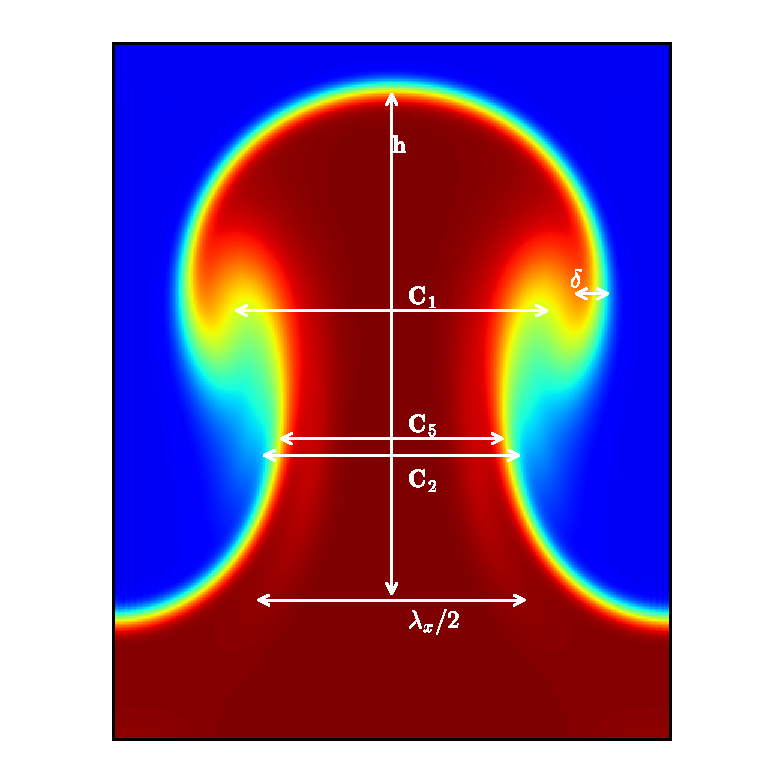
\includegraphics[width=\columnwidth]{figs/slice}
\caption{Scalar $\phi$}
\end{subfigure}
\begin{subfigure}[b]{\columnwidth}
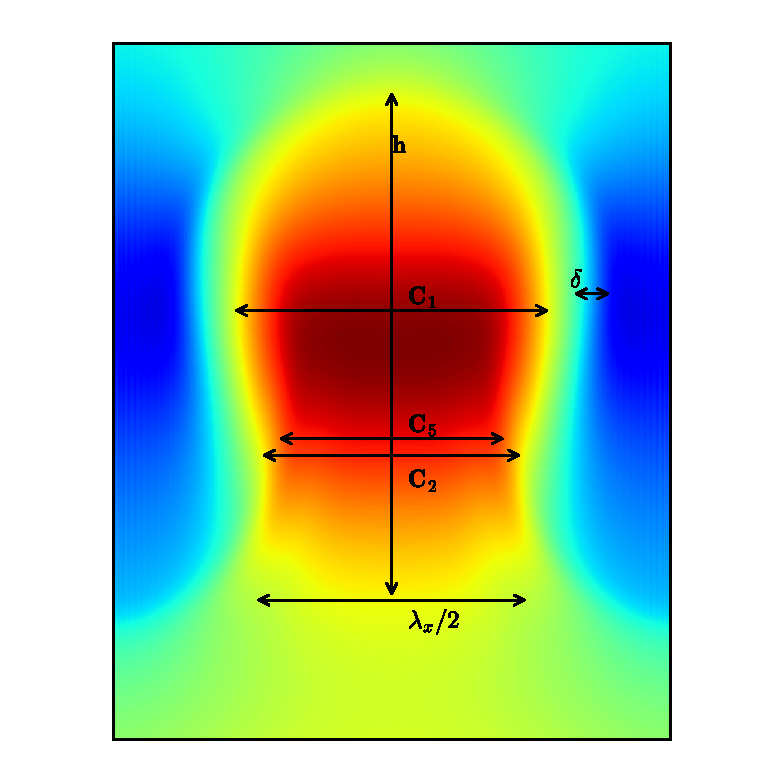
\includegraphics[width=\columnwidth]{figs/slice_w}
\caption{Vertical component of the velocity, $w$}
\end{subfigure}
\caption{ \flabel{bubble_geom}
Slices of the scalar and vertical component of the velocity along the diagonal of a bubble at early times and high Grashof number.
The arrows indiciate the dependence of the model terms on different span-wise length scales, and are identical in both figures.
$C_1$ is related to the maximum cross sectional diameter of the bubble in the velocity field.
$C_2$ is related to the nominal side-wall diameter of the bubble in the velocity field.
$C_5$ is related to the nominal side-wall diameter of the bubble in the scalar field.
$\delta$ is related to the interface thickness in the scalar field.
}
\end{figure*}

The parameter $C_1$ scales the form drag and serves as a drag coefficient.  
Because we have let $C_0 = 1$, the force balance is really aggreated over two rising bubbles and two falling spikes, each with diameter $\lambda / 2$.
Therefore, we multiply the force on a single bubble of diameter $\lambda/2$ by 4.
Now, we relate $C_1$ to the drag coefficient $C_d$ in the drag equation:
\begin{equation}
C_1 \lambda^2 \dot{h}^2 = 2 C_d A \dot{h}^2
\end{equation}
so $C_1$ can be estimated using drag coefficients of similar objects:
\begin{equation} \elabel{prior_c1}
C_1 = 2 C_d \frac{A}{\lambda^2},
\end{equation}
where $A \approx (\lambda/2)^2$.
Initially, the bubble tip is a flat plate, which has $C_d = 1.28$.
At late times, the bubble is closer to an elongated cylinder, which has $C_d = 0.82$, but with a somewhat streamlined tip, which further reduces drag.
We expect $C_1 \approx 0.64$, but possibly much smaller if the bubble takes a streamlined shape.
However, if the bubble spreads to have a diameter greater than $\lambda / 2$, $C_1$ could be greater than $0.64$.

Next, onsider the limit when $h \rightarrow \infty$ and $D = 0$:
The dynamical equation becomes
\begin{equation}
\ddot{h} = \frac{A g - C_2 \nu (1/\lambda) \dot{h}}{C_3}
\end{equation}
which leads to a terminal velocity of:
\begin{equation} \elabel{visc_vel}
\dot{h} = \frac{A g \lambda^2 }{C_2 \nu},
\end{equation}
or a non-dimensional velocity, i.e. Froude number:
\begin{equation}
\text{Fr} = \frac{d z}{d \tau} = \frac{\sqrt{\text{Gr}}}{C_2}.
\end{equation}
The case of extended bubbles and spikes affected only by viscous drag is highly analogous to flow through a square duct.
The pressure drop, $\Delta p$, along a duct is given by the Darcey-Weisbach formula:
\begin{equation}
\Delta p = \frac{f_D}{2} \frac{v^2 L}{d},
\end{equation}
where $L$ is the length of the duct,
$v$ is the mean velocity,
$d$ is the hydraulic diameter,
and $f_D$ is the Darcy friction factor.
In our case, $L = h$, $v = \dot{h}$, and $\Delta p = A g h$, so:
\begin{equation}
A g = \frac{f_D}{2} \frac{\dot{h}^2}{d},
\end{equation}
For laminar flows in circular pipes, $f_D = \bar{f}_D = 64 / \text{Re}$, so:
\begin{equation}
A g = \frac{f_D}{\bar{f}_D} 32 \nu \frac{\dot{h}}{d^2}.
\end{equation}
The hydraulic diameter $d = \lambda / 2$, so:
\begin{equation}
\dot{h} = \frac{\bar{f}_D}{f_D} \frac{A g \lambda^2}{128 \nu} .
\end{equation}
This gives an estimate for $C_2$:
\begin{equation}
C_2 \approx 128 \frac{f_D}{\bar{f}_D},
\end{equation}
where the ratio $f_D / \bar{f}_D$ is affected by the geometry and departure from laminar flow.
For example, for square ducts $f_D/\bar{f}_D \approx 0.889$, so $C_2 \approx 114.$. 

The product of the coefficient $C_5$ and $\lambda h$ gives the interfacial area of the side of the bubble.
Therefore, $C_5$ captures information both about the bubble shape and the bubble diameter.
If the bubbles had diameter $\lambda / 2$ and were smooth and rectangular, then $C_5 \approx 4$
If the bubble has a lower surface area shape, e.g. cylindrical, or is thinner then $C_5 < 4$.

These diameters, along with the relevant span-wise length scales in the preceeding coefficients, are sketched in \fref{bubble_geom}.
The diameter associated with $C_1$ is defined as the entrainment width at the bubble tip, in contrast to the width at the bubble center used for $C_2$.
The diameter associated with $C_5$ is defined similarly to $C_2$, but with respect to the scalar interface.
The interface width $\delta$ also depends on the scalar representation of the bubble.


\section{Conclusions}

We have proposed a simple ODE model for the growth of single mode Rayleigh-Taylor bubbles and spikes at low Atwood number.
The model targets an intermediate range of Reynolds numbers and high Peclet number, in which the single mode pertubration grows into an array of coherent bubbles and spikes.
The dynamics of the bubbles are described by a force balance between bouyancy, viscous drag, and form drag.
The buoyant force is scaled by a mixing factor related to the volume faction of mixed fluid within the bubble, which is modeled by diffusion across the bubble's interface.

The viscous drag, which is absent in other buoyancy-drag models, is essential to recovering terminal behavior at high aspect ratios and low diffusivities.  
Without viscous drag or mixing, the buoyant force grows with the aspect ratio while the form drag does not, leading to unbounded bubble velocity.
In practice, as the velocity grows, the bubble interface breaks up leading to enhanced turbulent mixing.

The ODE has 6 parameters, 3 of which can be constrained by limiting cases.
The immiscible linear theory, miscibile linear theory, and Poissile flow limits provide constraints.
The three remaining parameters lend themselves to physical interpretation, providing a guidline for their value.

To validate the simple model under its three constraints, we perform a battery of direct numerical simulations at moderate Reynolds number, high Peclet number, and high aspect ratio.
The simulations provide trajectories for the bubble height and volume of mixed fluid, which are directly compared to the results of the simple model.
Unconstrained, the model is able to reproduce the non-dimensional bubble height to one part in ???.
Constrained by the three limiting cases, the error increases to ???.
This demonstrates the compatability of the constraints with the model.

While the simple model is sufficient to describe coherent, steady bubbles and spikes at low Atwood numbers and high Peclet numbers, few real flows fall within this regime.
In this regard, the simple model proposed here is best seen as a starting point for extensions to more realistic flows.





\bibliography{library}

\end{document}

